\documentclass[letterpaper,12pt]{article}
\usepackage[utf8]{inputenc}
\usepackage[spanish,es-tabla]{babel}
\decimalpoint
\usepackage{amsfonts}
\usepackage{float}
\usepackage{mathptmx}
\usepackage{booktabs}

%\usepackage{heuristica}
%\usepackage[heuristica,vvarbb,bigdelims]{newtxmath}
\usepackage{graphicx}
\graphicspath{ {./} }

\usepackage{libertinus}
\usepackage[T1]{fontenc}

\usepackage[margin=1.3in]{geometry}
\usepackage{amsthm}
\usepackage{marvosym}
\usepackage{bm}

\renewcommand\qedsymbol{\Squarepipe}

\theoremstyle{definition}
\newtheorem{definition}{Definición}[section]
\newtheorem*{thm}{Teorema}


\setlength\parindent{0pt}

\newcounter{paragraphnumber}
\newcommand{\para}{%
  \vspace{10pt}\noindent{\bfseries\refstepcounter{paragraphnumber}\theparagraphnumber.\quad}%
}

%\setsecheadstyle{\large\bfseries}
%\setsubsecheadstyle{\bfseries}

\setlength\parindent{0pt}

\pagenumbering{gobble}


\usepackage{enumitem}
\setlist{nosep}

\usepackage{xcolor}

\usepackage{hyperref}
\hypersetup{
  colorlinks,
  linkcolor={red!50!black},
  citecolor={blue!50!black},
  urlcolor={green!50!black}
}

\usepackage{amssymb}
\usepackage{amsmath}

\begin{document}



\begin{center}
  {\large Aprendizaje Automatizado}\\
  \vspace{0.2cm}
  {\large\bfseries Tarea 4: Gráficos Probabilísticos}\\
  \vspace{0.2cm}
  {\large PCIC - UNAM}\\
  \vspace{0.5cm}
  {\itshape 20 de mayo de 2020}\\
  \vspace{0.5cm}
  Diego de Jesús Isla López\\
  (\href{mailto:dislalopez@gmail.com}{\itshape dislalopez@gmail.com})\\
  (\href{mailto:diego.isla@comunidad.unam.mx}{\itshape diego.isla@comunidad.unam.mx})\\
\end{center}


\section*{Ejercicio 1}

Se tienen las siguientes variables:

\begin{table}[H]
  \centering
  \begin{tabular}{|c|c|}
    \toprule
    Variable & Dominio \\
    \midrule
    \(A\) (alarma) & \{0,1\} \\
    \(D_A\) (alarma defectuosa) & \{0,1\} \\
    \(D_I\) (indicador defectuoso) & \{0,1\} \\
    \( I \) (lectura del indicador) & \(\mathbb{Z}\) \\
    \( T \) (temperatura real) & \(\mathbb{Z}\) \\
    \bottomrule
  \end{tabular}
\end{table}

\subsection*{Primer modelo}

La gráfica para el primer modelo es la siguiente: \\
\begin{figure}[H]
	\centering
	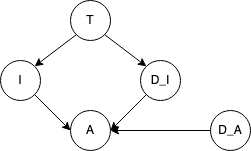
\includegraphics{m1}
\end{figure}
	

La probabilidad conjunta del modelo queda expresada como:

\begin{equation}
  P(T,I,D_I,A,D_A) = P(T)\cdot P(I|T) \cdot P(A|I) \cdot P(D_I|T)\cdot P(A|D_A,D_I,I) \cdot P(D_A) 
\end{equation}

En este modelo se busca representar el efecto de la temperatura sobre las variables \(I\) y \(D_I\), siendo \(A\) influenciada por estas dos además de \(D_A\).\\

Calculando el número de variables tenemos:

\begin{itemize}
	\item \(P(T) = 100\)
	\item \(P(D_A) = 2\)
	\item \(P(I|T) = 100 * 100 = 10000\)
	\item \(P(D_I|T) = 2 * 100 = 200\)
	\item \(P(A|D_A,D_I,I) = 2 * 100 * 2 * 2 = 800\)
	\item Total = 11102
\end{itemize}




\subsection*{Segundo modelo}

La gráfica para el segundo modelo es la siguiente: \\
\begin{figure}[H]
	\centering
	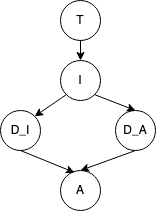
\includegraphics{m2}
\end{figure}


La probabilidad conjunta del modelo queda expresada como:

\begin{equation}
P(T,I,D_I,A,D_A) = P(T)\cdot P(I|T) \cdot P(D_A|I) \cdot P(D_I|I)\cdot P(A|D_A,D_I)
\end{equation}

Este modelo es similar al anterior, pero en este caso \(I\) influye directamente sobre \(D_A\) y \(D_I\) y estas a su vez influyen directamente en \(A\).

Calculando el número de variables tenemos:

\begin{itemize}
	\item \(P(T) = 100\)
	\item \(P(I|T) = 100 * 100 = 10000\)
	\item \(P(D_I|I) = 2 * 100 = 200\)
	\item \(P(D_A|I) = 2 * 100 = 200\)
	\item \(P(A|D_A,D_I) = 2 * 2 * 2 = 8\)
	\item Total = 10508
\end{itemize}



\subsection*{Tercer modelo}

La gráfica para este modelo es la siguiente: \\

\begin{figure}[H]
	\centering
	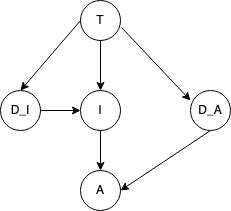
\includegraphics{m3}
\end{figure}


La probabilidad conjunta del modelo queda expresada como:

\begin{equation}
P(T,I,D_I,A,D_A) = P(T)\cdot P(D_I|T) \cdot P(I|D_IT) \cdot P(D_A|T)\cdot P(A|I,D_A)
\end{equation}

En este modelo se representa la influencia de la temperatura sobre la lectura del indicador, además de la posibilidad de que tanto la alarma y el indicador estén defectuosos, influyendo sobre la alarma a través de la lectura del indicador y la posibilidad de defecto de la alarma.

Calculando el número de variables tenemos:

\begin{itemize}
	\item \(P(T) = 100\)
	\item \(P(I|D_I,T) = 100 * 100 * 2 = 20000\)
	\item \(P(D_I|T) = 2 * 100 = 200\)
	\item \(P(D_A|T) = 2 * 100 = 200\)
	\item \(P(A|I,D_A) = 2 * 100 * 2 = 400\)
	\item Total: 20900
\end{itemize}


\section*{Ejercicio 2}

Para cada caso:

\subsection*{\(T  \perp\!\!\!\perp F | D\)}

Se tienen los caminos \(\{T,O,C,F\}\) y  \(\{T,O,D,B,F\}\).\\

Para el camino \(\{T,O,C,F\}\) tenemos las tripletas  \(\{T,O,C\}\) y \(\{O,C,F\}\). La tripleta \(\{T,O,C\}\) es activa ya que es una causa común de la que deriva la variable observada \(D\). La tripleta \(\{O,C,F\}\) representa una cadena causal y dado que ninguna de sus variables es observada, se considera como activa. \\

El camino  \(\{T,O,D,B,F\}\) es bloqueado dado que contiene a la variable observada, sin embargo ninguna de las tripletas del camino anterior resultan afectadas. \\

Por lo tanto, se tiene que \(T  \not\perp\!\!\!\perp F | D\).

\subsection*{\(C  \perp\!\!\!\perp B | F\)}

Se tienen los caminos \(\{C,F,B\}\) y \(\{C,O,D,B\}\).\\

El camino  \(\{C,F,B\}\) es inactivo ya que es una causa común derivada de la variable observada \(F\).\\

El camino \(\{C,O,D,B\}\) tiene las tripletas \(\{C,O,D\}\) y \(\{O,D,B\}\). La tripleta  \(\{C,O,D\}\) está activa ya que representa una cadena causal donde no hay variables observadas. Por su parte, la tripleta \(\{O,D,B\}\) representa un efecto común donde ninguna variable es observada, por lo que se considera inactiva. Ya que solo una de las tripletas está activa, el camino se considera inactivo.\\

Dado que no existen caminos activos, se sigue que \(C \perp\!\!\!\perp B | F\)

\subsection*{\(A  \perp\!\!\!\perp F | C\)}

Se tienen los caminos \(\{A,T,O,C,F\}\) y \(\{A,T,O,D,B,F\}\)

Para el camino \(\{A,T,O,C,F\}\) se tienen las tripletas \(\{A,T,O\}\)  y \(\{O,C,F\}\). La tripleta \(\{A,T,O\}\) es una cadena causal que no tiene variables observadas, por lo que está activa. La tripleta \(\{O,C,F\}\) es una cadena causal donde se observa la variable \(C\) por lo cual es inactiva. Por lo tanto, este camino es inactivo.\\


El camino  \(\{A,T,O,D,B,F\}\) cuenta con las tripletas  \(\{A,T,O\}\), \(\{O,D,B\}\) y  \(\{D,B,F\}\). La tripleta  \(\{O,D,B\}\) es inactiva ya que representa una causa común sin variables observadas.

Como ambos caminos son inactivos, se sostiene que \(A  \perp\!\!\!\perp F | C\).

\subsection*{\(A  \perp\!\!\!\perp F | C,D\)}

Se tienen nuevamente los caminos \(\{A,T,O,C,F\}\) y \(\{A,T,O,D,B,F\}\).\\

El camino  \(\{A,T,O,D,B,F\}\) es activo puesto que todas las tripletas son activas. Las tripletas \(\{A,T,O\}\) y \(\{T,O,D\}\) son cadenas causales sin variables observadas. La tripleta \(\{D,B,F\}\) también representa una cadena causal activa, aunque contiene a la variable observada \(D\), ya que esta se encuentra al final de la cadena.\\

Dado que existe al menos un camino activo, se sigue que \(A  \not\perp\!\!\!\perp F | C,D\)


\section*{Ejercicio 3}

\subsection*{Escribe la distribución conjunta de la red bayesiana en función de las probabilidades condicionales}

La distribución conjunta de la red queda expresada como:

\begin{equation}
P(E,F,S,V,C,D) = P(E) \cdot P(F|E) \cdot P(S|E) \cdot P(V|F,S) \cdot P(C|S) \cdot P(D|V)
\end{equation}

\subsection*{Si un paciente es llevado al doctor, usando un paquete de software calcula la probabilidad de que no tenga ébola}

Para este ejercicio se utiliza la biblioteca pgmpy. El código fuente se encuentra adjunto a este documento.\\

El resultado encontrado es:

\begin{table}[H]
	\centering
	\begin{tabular}{|c|c|}
		\toprule
		Ebola & P(Ebola) \\
		\midrule
		Ebola = T & 0.0752 \\
		Ebola = F & 0.9248  \\
		\bottomrule
	\end{tabular}
\end{table}

Por lo tanto, la probabilidad de que el paciente no tenga ébola dado que fue llevado al doctor es de 92.48\%.


\subsection*{Convierte la red bayesiana en un modelo gráfico no dirigido (campo aleatorio de Markov) y dibújalo. Captura tantas relaciones de independencia condicional como sea posible}

El modelo queda expresado por el siguiente campo aleatorio de Markov:

\begin{figure}[H]
	\centering	
	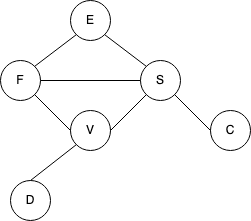
\includegraphics{markov}
	\caption{Representación del problema mediante un campo aleatorio de Markov}	
\end{figure}

Las probabilidades condicionales que podemos encontrar en el modelo son:\\

\begin{itemize}
	\item Si \(S\) es observada, podemos ver que \(C\) queda desconectada de la gráfica, teniendo así:
	\begin{enumerate}
		\item \(E \perp\!\!\!\perp C|S \)
		\item \(F \perp\!\!\!\perp C|S \)
		\item \(V \perp\!\!\!\perp C|S \)
		\item \(D \perp\!\!\!\perp C|S \)
	\end{enumerate}
	
	\item Si \(V\) es observada, podemos ver que \(D\) queda desconectada de la gráfica, teniendo así:
	\begin{enumerate}
		\item \(E \perp\!\!\!\perp D|V \)
		\item \(F \perp\!\!\!\perp D|V \)
		\item \(S \perp\!\!\!\perp D|V \)
		\item \(C \perp\!\!\!\perp D|V \)
	\end{enumerate}

	\item Finalmente si  \(S\) y \(F\) son observadas, podemos ver que \(E\) y \(C\) quedan desconectadas de la gráfica, teniendo así:
	\begin{enumerate}
		\item \(V \perp\!\!\!\perp C|F,S \)
		\item \(D \perp\!\!\!\perp C|F,S \)
		\item \(V \perp\!\!\!\perp E|F,S \)
		\item \(D \perp\!\!\!\perp E|F,S \)
		\item \(E \perp\!\!\!\perp C|F,S \)
		\item \(C \perp\!\!\!\perp E|F,S \)
	\end{enumerate}
\end{itemize}

\subsection*{Debido a una campaña de concientización de la salud, las personas son alentadas a visitar la clínica en caso de que tengan fiebre. Esto incrementa la cantidad de visitas de personas con fiebre sin importar el estado de cualquier otra variable.}

\textbf{1. ¿Qué probabilidades condicionales en la red se modifican debido a este cambio y en qué sentido?}\\

Hay probabilidades que aumentarán y otras que disminuirán. Las probabilidades que aumentan son:\\

\begin{itemize}
	\item \(P(V=\texttt{verdadero}|F=\texttt{verdadero},S=\texttt{verdadero})\)
	\item \(P(V=\texttt{verdadero}|F=\texttt{verdadero},S=\texttt{falso})\)
\end{itemize}
\medskip
Esto es debido a que las visitas aumentarán independientemente de la presencia de sangrado en el paciente. Por ende, disminuirá la probabilidad de que el paciente no asista a la clínica a pesar de tener fiebre (\(P(V=\texttt{falso}|F=\texttt{verdadero},S)\)).

\medskip

\textbf{2. Describe cualquier otro efecto que esto tenga en la proporción de personas con complicaciones que visiten la clínica. Menciona exactamente qué probabilidades condicionales usaste para llegar a tu conclusión.}

\medskip

Observando el modelo, la aparición de complicaciones depende directamente de la presencia de sangrado en el paciente. Esto es:

\begin{itemize}
	\item \( P(C = \texttt{verdadero} | S = \texttt{verdadero}) = 0.75 \)
	\item \( P(C = \texttt{verdadero} | S = \texttt{verdadero}) = 0.1 \)
\end{itemize}

De esta manera podemos ver que la diferencia es significativa para los casos en los que existe sangrado y los que no. Sin embargo, se espera que las visitas aumenten debido a la campaña, la cual está basada en la presencia de fiebre. Dado que los demás síntomas son irrelevantes para la campaña, se espera que aumente el número de pacientes que presentan tanto fiebre como sangrado.

\subsection*{Asume que alguien que no tiene fiebre va al doctor, ¿qué relación de independencia condicional existe en la distribución que no puede ser descubierta a través del grafo solamente?}

Poniendo el enunciado en términos de independencia condicional, buscamos demostrar que:

\begin{equation}
E \perp\!\!\!\perp V | F = \texttt{falso}, D = \texttt{verdadero}
\end{equation}

Observando el gráfico, es posible ver que entre \(E\) y \(V\)) existen dos caminos, los cuales consisten de una sola tripleta cada uno: \(\{E,F,V\}\) y  \(\{E,S,V\}\). Ambos caminos son cadenas causales; de esta manera el camino \(\{E,F,V\}\) es inactivo puesto que la variable \(F\) es observada y está en el medio. Por su parte, el camino  \(\{E,S,V\}\) es activo puesto que no contiene ninguna variable observada. Entonces, se concluye que no es posible demostrar este caso de independencia mediante el modelo gráfico. \\

Usando marginalización tenemos que: 

\begin{align*}
P(E,V | F = \texttt{falso},D = \texttt{verdadero}) = & P(E|F = \texttt{falso},D = \texttt{verdadero}) \\
                             & \cdot P(V|\texttt{falso},D = \texttt{verdadero})
\end{align*}

Esto es, \(\forall e,v \in \{\texttt{verdadero},\texttt{falso}\}\):

\begin{align*}
P(e,v|\texttt{falso},D = \texttt{verdadero}) = & P(e|F = \texttt{falso},D = \texttt{verdadero}) \\
&  \cdot P(v|\texttt{falso},D = \texttt{verdadero})
\end{align*}


Utilizando pgmpy encontramos la solución:\\

\begin{table}[H]
	\centering
	\begin{tabular}{|c|c|}
		\toprule
		Ebola & P(Ebola) \\
		\midrule
		Ebola = T & 0.0670 \\
		Ebola = F & 0.9330  \\
		\bottomrule
	\end{tabular}
\end{table}


\begin{table}[H]
	\centering
	\begin{tabular}{|c|c|}
		\toprule
		Visita & P(Visita) \\
		\midrule
		Visita = T & 1 \\
		Visita = F & 0  \\
		\bottomrule
	\end{tabular}
\end{table}

\begin{table}[H]
	\centering
	\begin{tabular}{|c|c|}
		\toprule
		Ebola,Visita & P(Ebola,Visita) \\
		\midrule
		Ebola = T,Visita = T & 0.0670 \\
		Ebola = F, Visita = T & 0  \\
		Ebola = T, Visita = F & 0.9330  \\
		Ebola = F, Visita = F & 0  \\
		\bottomrule
	\end{tabular}
\end{table}


\subsection*{Problema opcional}

Sabemos que la probabilidad condicional está expresada por:


\begin{equation*}
P(E,F,S,V,C,D) = P(E) \cdot P(F|E) \cdot P(S|E) \cdot P(V|F,S) \cdot P(C|S) \cdot P(D|V)
\end{equation*}

De este modo, las variables ocultas para este problema son \(F\), \(S\), \(C\) y \(D\). Primero obtenemos las tablas de valores para cada variable:

\begin{table}[H]
	\centering
	\begin{tabular}{|c|c|}
		\toprule
		E & P(E) \\
		\midrule
		E = T & 0.01 \\
		E = F,& 0.99  \\
		\bottomrule
	\end{tabular}
	\caption{Valores para E}
\end{table}


\begin{table}[H]
	\centering
	\begin{tabular}{|c|c|}
		\toprule
		E,F & P(F|D) \\
		\midrule
		E = verdadero, F = verdadero & 0.6 \\
		E = verdadero, F = falso & 0.4  \\
		E = falso, F = verdadero & 0.1  \\
		E = falso, F = falso & 0.9  \\
		\bottomrule
	\end{tabular}
	\caption{Valores para F|E}
\end{table}

\begin{table}[H]
	\centering
	\begin{tabular}{|c|c|}
		\toprule
		E,S & P(S|E) \\
		\midrule
		E = verdadero, S = verdadero & 0.8 \\
		E = verdadero, S = falso & 0.2 \\
		E = falso, S = verdadero & 0.05  \\
		E = falso, S = falso & 0.95  \\
		\bottomrule
	\end{tabular}
	\caption{Valores para S|E}
\end{table}


\begin{table}[H]
	\centering
	\begin{tabular}{|c|c|}
		\toprule
		F,S,V & P(V|F,S) \\
		\midrule
		F = verdadero, S = verdadero, V = verdadero & 0.8 \\
		F = verdadero, S = verdadero, V = falso     & 0.2  \\
		F = verdadero, S = falso, V = verdadero     & 0.5 \\
		F = verdadero, S = falso, V = falso        & 0.5  \\
		F = falso, S = verdadero, V = verdadero & 0.7 \\
		F = falso, S = verdadero, V = falso     & 0.3  \\
		F = falso, S = falso, V = verdadero     & 0 \\
		F = falso, S = falso, V = falso        & 1  \\
		\bottomrule
	\end{tabular}
	\caption{Valores para V|F,S}
\end{table}

\begin{table}[H]
	\centering
	\begin{tabular}{|c|c|}
		\toprule
		S,C & P(C|S) \\
		\midrule
		S = verdadero, C = verdadero & 0.75 \\
		S = verdadero, C = falso & 0.25 \\
		S = falso, C = verdadero & 0.1  \\
		S = falso, C = falso & 0.9  \\
		\bottomrule
	\end{tabular}
	\caption{Valores para C|S}
\end{table}

\begin{table}[H]
	\centering
	\begin{tabular}{|c|c|}
		\toprule
		V,D & P(D|V) \\
		\midrule
		V = verdadero, D = verdadero & 0.6 \\
		V = verdadero, D = falso & 0.4 \\
		V = falso, D = verdadero & 0  \\
		V = falso, D = falso & 1  \\
		\bottomrule
	\end{tabular}
	\caption{Valores para D|V}
\end{table}

Marginalizando las variables ocultas, la probablidad se expresa como:

\begin{align*}
P(V,E=\text{verdadero})&=\\
\sum_{f}\sum_{s}\sum_{c}\sum_{d}[&P(E=\text{verdadero})P(f|E=\text{verdadero})P(s|E=\text{verdadero})P(V|f,s)P(c|s)P(d|V)]\\
\end{align*}


Reformulando, se obtiene:

\begin{align*}
P(V,E=\text{verdadero})&=\\
P(E=\text{verdadero})[\sum_{f}&\sum_{s}[P(f|E=\text{verdadero})P(s|E=\text{verdadero})P(V|f,s)\sum_{c}[P(c|s)]\sum_{d}[P(d|V)]]]\\
\end{align*}


Para eliminar \(D\) obtenemos \(F_d(V) = \sum_{d}[P(d|V)]\):

\begin{table}[H]
	\centering
	\begin{tabular}{|c|c|}
		\toprule
		V & \(F_d(V)\) \\
		\midrule
		verdadero & 0.6 + 0.4 = 1 \\
		falso & 0 + 1  = 1 \\
		\bottomrule
	\end{tabular}
	\caption{Valores para \(F_d(V)\)}
\end{table}


En este paso, la ecuación queda:

\begin{align*}
	P(V,E=\texttt{verdadero})&=\\
	P(E=\texttt{verdadero})[\sum_{f}&\sum_{s}[P(f|E=\text{verdadero})P(s|E=\text{verdadero})P(V|f,s)\sum_{c}[P(c|s)]F_d(V)]]\\
\end{align*}

Para eliminar \(C\) obtenemos \(F_c(s) = \sum_{c}[P(c|s)]\):

\begin{table}[H]
	\centering
	\begin{tabular}{|c|c|}
		\toprule
		S & \(F_c(s)\) \\
		\midrule
		verdadero & 0.75 + 0.25 = 1 \\
		falso & 0.1 + 0.9  = 1 \\
		\bottomrule
	\end{tabular}
	\caption{Valores para \(F_c(s)\)}
\end{table}


En este paso, la ecuación queda:

\begin{align*}
P(V,E=\text{verdadero})& = \\
& P(E=\text{verdadero})[\sum_{f}[P(f|E=\text{verdadero})\sum_{s}[P(s|E=\text{verdadero})P(V|f,s)F_c(s)]F_d(V)]]\\
\end{align*}


Para eliminar \(S\) obtenemos \(F_s(V,f) = \sum_{s}[P(f|E=\text{verdadero})P(s|E=\text{verdadero})P(V|f,s)F_c(s)]\). Construyendo \(F_s(V,f)\):\\

\begin{table}[H]
	\centering
	\begin{tabular}{|c|c|c|c|}
		\toprule
		S & V & F & \(P(s|E=\text{verdadero})P(V|f,s)F_c(s)\) \\
		\midrule
		verdadero & verdadero & verdadero & 0.64 \\
		verdadero & verdadero & falso & 0.56 \\
		verdadero & falso & verdadero & 0.16 \\
		verdadero & falso & falso & 0.24 \\
		falso & verdadero & verdadero & 0.1 \\
		falso & verdadero & falso & 0 \\
		falso & falso & verdadero & 0.1 \\
		falso & falso & falso & 0.2 \\
		\bottomrule
	\end{tabular}
	\caption{Construcción \(F_s(V,f)\)}
\end{table}

Así, calculamos:\\

\begin{table}[H]
	\centering
	\begin{tabular}{|c|c|c|}
		\toprule
		V & F &  \(F_s(V,f)\) \\
		\midrule
		verdadero & verdadero & 0.74 \\
		verdadero & falso & 0.56\\
		falso & verdadero & 0.26\\
		falso & falso & 0.44\\
		\bottomrule
	\end{tabular}
	\caption{Valores para \(F_s(V,f)\)}
\end{table}


En este paso, la ecuación queda:

\begin{align*}
P(V,E=\texttt{verdadero})&=\\
&P(E=\texttt{verdadero})[\sum_{f}[P(f|E=\text{verdadero})F_s(V,f)]F_d(V)]
\end{align*}

Para eliminar \(F\) obtenemos \(F_f(V) = \sum_{f}[P(f|E=\text{verdadero})F_s(V,f)]\). Construyendo, tenemos:


\begin{table}[H]
	\centering
	\begin{tabular}{|c|c|c|}
		\toprule
		F & V &  \(P(f|E=\texttt{verdadero})F_s(V,f)\) \\
		\midrule
		verdadero & verdadero & 0.444 \\
		verdadero & falso & 0.156\\
		falso & verdadero & 0.224\\
		falso & falso & 0.176\\
		\bottomrule
	\end{tabular}
	\caption{Construcción para \(F_f(V)\)}
\end{table}

Así, el valor para \(F_f(V)\) queda:


\begin{table}[H]
	\centering
	\begin{tabular}{|c|c|}
		\toprule
		V &  \(F_f(V)\) \\
		\midrule
		verdadero  & 0.668 \\
		falso &  0.332\\
		\bottomrule
	\end{tabular}
	\caption{Valores para \(F_f(V)\)}
\end{table}

Finalmente la ecuación queda:

\begin{equation}
	P(V,E=\texttt{verdadero})=P(E=\texttt{verdadero})[F_f(V)F_d(V)]\\
\end{equation}

Entonces calculamos la probabilidad:

\begin{table}[H]
	\centering
	\begin{tabular}{|c|c|}
		\toprule
		V &  \(P(E=\texttt{verdadero})[F_f(V)F_d(V)]\) \\
		\midrule
		verdadero  & 0.00668 \\
		falso &  0.00332\\
		\bottomrule
	\end{tabular}
	\caption{Valores para \(P(V,E=\texttt{verdadero})\)}
\end{table}

Así, se tiene:

\begin{equation*}
P(V=\text{verdadero}|E=\text{verdadero})=\frac{0.00668}{0.00668+0.00332}= 0.668\\
\end{equation*}

\begin{equation*}
P(V=\text{falso}|E=\text{verdadero})=\frac{0.00332}{0.00668+0.00332}= 0.332\\
\end{equation*}
\end{document}

